\documentclass[a4paper,11pt]{article}
\usepackage[margin=2cm]{geometry}

\usepackage[nodayofweek]{datetime}
\usepackage{cite}
\usepackage{graphicx}
\longdate

\usepackage{hyperref}
\usepackage{fancyhdr}
\pagestyle{fancyplain}
\fancyhf{}
\lhead{\fancyplain{}{M.Sc.\ Group Project Report}}
\rhead{\fancyplain{}{\today}}
\cfoot{\fancyplain{}{\thepage}}


\title{Implementation of attentional bistability of the dragonfly visual neurons in an intelligent biomimetic agent\\\Large{--- Final Report ---}}
\author{Juan Carlos Farah, Panagiotis Almpouras, Ioannis Kasidakis, Erik Grabljevec, Christos Kaplanis\\
       \{jcf214, pa512, ik311, eg1114, ck2714\}@doc.ic.ac.uk\\ \\
       \small{Supervisors: Professor Murray Shanahan, Zafeirios Fountas, Pedro Mediano}\\
       \small{Course: CO530/533, Imperial College London}
}

\begin{document}
\maketitle

\section{Design}

The challenge of designing a tool that could satisfy the overall functionality outlined in the introduction could be distilled down to two main facets:
\begin{enumerate}
\item Deciding on the components of the dragonfly visual system and how they would be connected together.
\item Deciding on the user interface and specifying an API for the system.
\end{enumerate}

\subsection{Components}

Having consulted academic research on the subject of dragonfly vision and discussed with our supervisors, we managed to identify five key components we would need to model in order to implement a coherent system. 

\begin{enumerate}
\item{Target Animation:} An animated video that provides the visual input to the system, emulating the retina of the dragonfly. User should be able to specify movements of multiple targets within the visual field and choose the background.
\item{Elementary Small Target Motion Detector (ESTMD):} The ESTMD neurons are the first layer of visual processing in the dragonfly. They have the general function of identifying and isolating small moving targets, even against a cluttered, moving background (WIEDERMAN 2008). They take arrays of pixel values as input from the animation and output firing rates of neurons to be processed by the next layer.
\item{Centrifugal Small Target Motion Detector (CSTMD):} The CSTMD neuron is a higher order visual neuron in the brain of the dragonfly. This neuron reacts to the presentation of multiple visual stimuli by firing as if only one of the stimuli was present \cite{w13}. The CSTMD takes the firing rates of the ESTMD as input and outputs a time series of neuron spikes (spike trains) to the next layer.
\item{Pattern Recognition:} This module has the function of detecting patterns in the output of the CSTMD in order to distil features of target movement within the visual field. While it does not have a direct correspondence to a layer of neurons in the dragonfly, it uses a well-established biological learning mechanism called Spike Timing Dependent Plasticity (STDP) \cite{stdp1}\cite{stdp2}. It outputs spike trains to the Action Selection module.
\item{Action Selection:} This model converts the output of the pattern recognition neurons into movement of the dragonfly, emulating the connection between the visual processing to the motor neurons. It can be trained using STDP combined with reward modulation so that the dragonfly learns to maximise target capture based on the patterns in its visual field. The final output is the original animation with the position of the dragonfly superimposed onto each frame for observation of how effectively it chases targets.
\end{enumerate}

\subsection{User Interface}
For the user interface we decided that a web client would be the most suitable solution. The web client is designed to be a simple interface that allows for simulations for each of the modules to be run and automated, either separately or jointly. This graphical user interface interacts with each module's API and provides the functionality needed to save and access the results of every experiment. It provides key metrics that can be crucial in understanding the performance of the system.
Given the computationally expensive nature of our modules' simulations, a persistent store had to be used to save the output and results of each run. As shown in the structure diagram below, the five modules that our project comprises, are connected sequentially. Saving the output of each module enabled us to reuse the output of a module as input to the next, multiple times without the need to rerun any of the previous modules. What is more, the persistent store allows the web client to provide a view of the results for analysis simply by querying the database instead of regenerating them each time.
For our data store MongoDB was chosen. MongoDB provides a fast, scalable solution that does not require strict design decisions in advance. Considering in retrospect the changes and adaptations that had to take place during this project, we trust that MongoDB was a wise choice that contributed to the overall success of this project.


\subsection{Design diagram}
The following figure provides a graphical representation of the system as whole. 

\begin{figure}[hb]
\centering
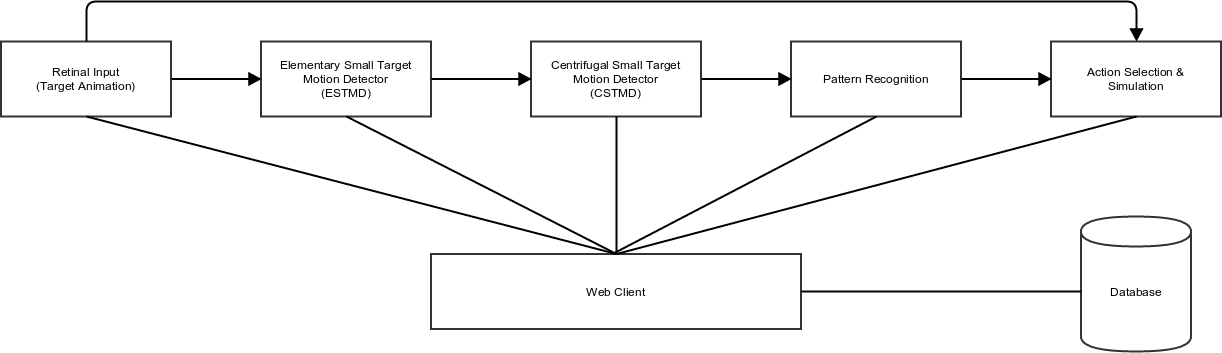
\includegraphics[scale = 0.35]{designblockdiagram2}
\caption{Project Structure Diagram.}
\end{figure}

\subsection{Programming language}
We decided that it made sense that the various modules were all programmed in the same language so that they could be easily linked into the web client. The programming language used throughout the project was Python \cite{python}. Python includes libraries that allow for efficient matrix manipulations that were key in most of the modules. Matlab was an alternative we initially considered \cite{matlab}. Although Matlab is very powerful and user friendly for some particular tasks, it does not allow for the flexibility that Python does. For that reason Matlab was disregarded as an option.
The database we used was MongoDB because of the increasing popularity of the distributed databases as well as the fact that this was the database scheme we were most familiar with.




\end{document}

